\documentclass[aps, letterpaper, onecolumn, superscriptaddress, notitlepage, 10pt]{revtex4-1}
\usepackage{times}

% use these settings for a more reader-friendly version
%\documentclass[aps, pra, a4paper, 11pt, onecolumn, nofootinbib, superscriptaddress, tightenlines, notitlepage, longbibliography]{revtex4-1}

%------------------------------------------------------------------------------------------------------------%
% Packages
%------------------------------------------------------------------------------------------------------------%

\usepackage{xcolor}
\usepackage{amsmath,amsfonts,amssymb}
\usepackage{graphicx}
\usepackage[caption=false]{subfig}
\usepackage{enumerate}
\usepackage{mathrsfs}
\usepackage{enumitem}

\usepackage{tikz}
\usetikzlibrary{decorations.pathreplacing,calc}

\usepackage[pdfpagelabels,pdftex,bookmarks,breaklinks]{hyperref}
\definecolor{darkblue}{RGB}{0,0,127} % choose colors
\definecolor{darkgreen}{RGB}{0,150,0}
\hypersetup{colorlinks, linkcolor=darkblue, citecolor=darkgreen, filecolor=red, urlcolor=blue}
\hypersetup{pdfauthor={Simon Burton, Courtney G. Brell, Steven T. Flammia}}
\hypersetup{pdftitle={Classical Simulation of Quantum Error Correction in a Fibonacci Anyon Code}}

\usepackage[normalem]{ulem}

%------------------------------------------------------------------------------------------------------------%
\begin{document}

\title{Supplemental material for ``Classical Simulation of Quantum Error Correction in a Fibonacci Anyon Code''}

\author{Simon Burton}
\affiliation{Centre for Engineered Quantum Systems, School of Physics, 
The University of Sydney, Sydney, Australia}
\author{Courtney G.\ Brell}
\affiliation{Institut f\"{u}r Theoretische Physik, Leibniz Universit\"{a}t Hannover, 
Appelstra\ss{}e 2, 30167 Hannover, Germany}
\affiliation{Perimeter Institute for Theoretical Physics, 
Waterloo, Canada}
\author{Steven T.\ Flammia}
\affiliation{Centre for Engineered Quantum Systems, School of Physics, 
The University of Sydney, Sydney, Australia}

\date{\today}

\maketitle

%------------------------------------------------------------------------------------------------------------%
% Macros
%------------------------------------------------------------------------------------------------------------%

\newcommand{\Eref}[1]{Eq.~(\ref{#1})}
\newcommand{\Fref}[1]{Fig.~\ref{#1}}
\newcommand{\Aref}[1]{Appendix~\ref{#1}}

\newcommand{\e}{\mathrm{e}}
\newcommand{\vac}{\mathbb{I}}

\newcommand{\ket}[1]{|{#1}\rangle}
\newcommand{\expect}[1]{\langle{#1}\rangle}
\newcommand{\bra}[1]{\langle{#1}|}
\newcommand{\ketbra}[2]{\ket{#1}\!\bra{#2}}
\newcommand{\braket}[2]{\langle{#1}|{#2}\rangle}
\newcommand{\proj}[1]{\ketbra{#1}{#1}}

\newcommand{\cggb}[1]{\textcolor{blue}{#1}}
\newcommand{\simon}[1]{\textcolor{red}{#1}}
\newcommand{\stf}[1]{\textcolor{green}{#1}}


\newcommand{\F}{\mathscr{H}} % H or F ?
\newcommand{\C}{\mathbb{C}}
\newcommand{\R}{\mathbb{R}}
\newcommand{\A}{\mathcal{A}}
\newcommand{\Hom}{{\mathrm{Hom}}}

\newcommand{\subsub}[1]{{\bf #1}}

%------------------------------------------------------------------------------------------------------------%

\newcommand{\ntikzmark}[2]{#2\thinspace\tikz[overlay,remember picture,baseline=(#1.base)]{\node[inner sep=0pt] (#1) {};}}

\newcommand{\makebrace}[3]{%
    \begin{tikzpicture}[overlay, remember picture]
        \draw [decoration={brace,amplitude=0.5em},decorate]
        let \p1=(#1), \p2=(#2) in
        ({max(\x1,\x2)}, {\y1+0.8em}) -- node[right=0.6em] {#3} ({max(\x1,\x2)}, {\y2});
    \end{tikzpicture}
}


In order to estimate the error-correction threshold of Fibonacci anyon codes, we perform monte-carlo simulations of noise and recovery operations on systems of various sizes. For a given sample, the simulation can be broken down into several stages:
\begin{itemize}[noitemsep, topsep=0pt]
\item \ntikzmark{N}{Noise}
\item \ntikzmark{S}{Syndrome extraction}
\item \ntikzmark{D}{Decoding}
\item \ntikzmark{R}{Recovery}
\end{itemize}
\makebrace{S}{R}{Error-correction}
After application of noise, the subsequent three steps (forming the error-correction routine) are iterated until success or failure, as will be described in more detail below.

It should be noted that while the noise, syndrome extraction, and recovery steps of this procedure are intended to really be a simulation of the physics of an anyon system, the decoding step is better thought of as an implementation of the classical processing that a successful error-correction experiment will require. Furthermore, the simulation of the noise and recovery steps will be rendered straightforward by the way we model our system in the first place. As such, the main novelty of our simulations is in the model itself, and the syndrome extraction step.

The key to simulating these processes effectively is the ability to describe topological operations by \emph{curve diagrams}. This is an alternative representation of topological operations that is particularly suited to these kinds of numerical simulations of sparsely populated 2-dimensional anyon systems. The theoretical framework underpinning this description and the relation to to other representations of topological operations is discussed in Ref.~\cite{Burton2016}.

In this supplementary material, we first describe our physical model of an anyon system and the corresponding noise, before showing how to simulate joint charge measurements (the core of syndrome extraction) within this model. The use of curve-diagrams is presented in an intuitive but ad-hoc way. Finally we describe our decoder and detail holistically how the different parts of the simulation interact.


\section{Physical model}

We consider anyon systems defined on a torus.
We endow this with a $L\times L$ square lattice of observables:
$$
    \Lambda := \bigl\{ \gamma_{ij} \bigr\}_{i,j=1,...,L}
$$
These observables are the physically accessible charge observables that will be measured during syndrome extraction, before being passed to the decoder which will in turn determine physical recovery operations to be performed on the system.

We call each $\gamma_{ij}$ a \emph{tile.}
In figures we show a small gap between the tiles but this is not meant
to reflect an actual physical gap.

As noted above, the key to our model is to represent anyons and topological operations with curve diagrams. A curve diagram is a directed path that connects several anyons, which are denoted by preferred points along these paths. A curve diagram specifies a linear ordering of the anyons that allows us to define a basis for the corresponding fusion space, as well as to keep track of topological operations on this ordering. See Ref.~\cite{Burton2016} for a more formal introduction to curve diagrams.

The main noise processes we consider in our simulations are pair-creation events, though other topological processes such as hopping, exchange, etc.~can also be implemented straightforwardly.
The pair-creation process acts to populate the manifold with
a randomly distributed set of anyon pairs,
whose separation is much smaller than the size of a tile.

Each such pair will have vacuum total charge and so the observables
$\gamma_{ij}$ will only be affected by pairs that cross a tile boundary, i.e.~we
need only consider distributing these pairs along edges of the tiles:
\begin{center}
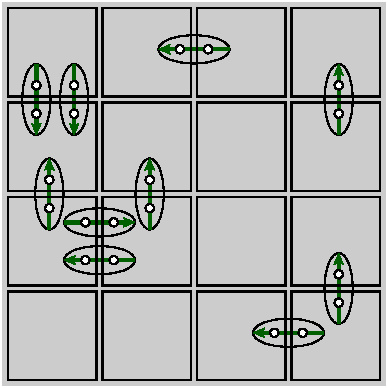
\includegraphics[width=0.3\columnwidth ]{pic-pair-create.pdf}
\end{center}

In simulating system undergoing noise for time $T$, we place a Poisson-distributed number of pair-creation events on the edges of tiles, with mean $2L^2T$.

In order to allow us to later calculate fusion outcomes for sets of anyons, in addition to locations of created anyons we also assign each pair a (directed) piece of curve, denoted in green. This curve can be thought of as a choice of fusion basis for the anyons along it. Since the total charge of any newly-created particle-antiparticle pair is vacuum, each of their fusion spaces can be treated independently. This results in our being able to consider independent disconnected curves for each such pair. We only need consider the joint state in the fusion space of different sets of anyons if they have interacted, and so it is with curve diagrams. Using this picture, it is easy to track the effects of moving anyons, which essentially are represented by appropriate extensions or deformations of the curve along which the anyon lies. These kinds of straightforward processes are all that are required to describe the noise and recovery steps of our simulation.


\section{Syndrome extraction}

Syndrome extraction in this model corresponds to simulating measurements of the observables $\gamma_{ij}$, which represent the total charge contained within the corresponding tile.

In order to compute measurement outcomes for the $\gamma_{ij}$
we first need to concatenate any two curve diagrams that 
participate in the same $\gamma_{ij}.$
Because each curve has vacuum total charge this can be
done in an arbitrary way:
\begin{center}
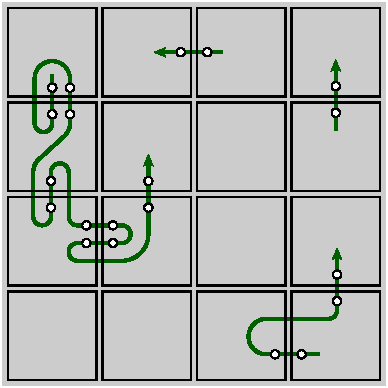
\includegraphics[width=0.3\columnwidth ]{pic-join-pairs.pdf}
\end{center}

Working in the basis picked out by the resulting curve
diagrams, we will show how to calculate measurement outcomes for each tile,
the result of which is recorded on the original curve:
\begin{center}
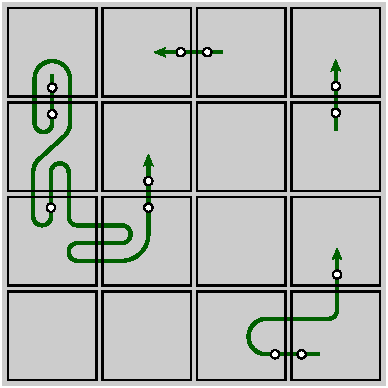
\includegraphics[width=0.3\columnwidth ]{pic-curve-uniq.pdf}
\end{center}

%
% ~~~~~~~~~~~~~~~~~~~~~~~~~~~~~~~~~~~~~~~~~~~~~~~~~~~~~~~~~~~~~~~~~~~~~~~~~~~~
%

The basic data structure involved in the
simulation we term a \emph{combinatorial curve diagram.}
Firstly, we will require each curve to intersect 
the edges of tiles transversally,
and in particular a curve will not touch a tile corner.

For each tile in the lattice,
we store a combinatorial
description of the curve(s) intersected with that tile.
Each component of such an intersection we call a \emph{piece-of-curve.}
\begin{center}
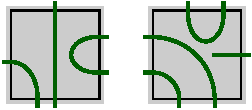
\includegraphics[]{pic-cells.pdf}
\end{center}

We follow essentially the same approach as taken in \cite{Abramsky2007} 
to describe elements of a Temperley-Leib algebra, but
with some extra decorations.
The key idea is to store a \emph{word} for each tile, comprised of
the letters $\bigl<$ and $\bigr>$.
Reading in a clockwise direction around the edge of
the tile from the top-left corner,
we record our encounters with each piece-of-curve,
writing~$\bigl<$ for the first encounter, and~$\bigr>$ for the
second.
We may also encounter a dangling piece-of-curve
(the head or the tail), so we use another symbol $*$ for this.
The words for the above two tiles will then be 
$\bigl<\bigl<\bigr>\bigr>\bigl<\bigr>$ and $\bigl<\bigr>*\bigl<\bigl<\bigr>\bigr>.$
When the brackets are balanced,
each such word will correspond one-to-one with an intersection
of a curve in a tile, up to a continuous deformation of the interior of the tile.
Ie. the data structure 
will be insensitive to any continuous deformation of the interior of the tile,
but the simulation does not need to track any of these degrees of freedom.

\begin{center}
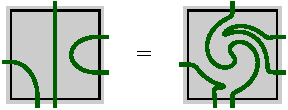
\includegraphics[]{pic-cells-0.pdf}
\end{center}

We will also need to record
various other attributes of these curves,
and to do this we make this notation more elaborate
in the paragraphs {\bf (I)}, {\bf(II)} and {\bf(III)} below.
Each symbol in the word describes an intersection of
the curve with the tile boundary,
and so as we decorate these symbols these decorations will
apply to such intersection points.

\begin{center}
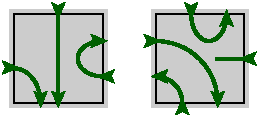
\includegraphics[]{pic-cells-1.pdf}
\end{center}

{\bf (I)} We will record the direction of each piece-of-curve,
this will be either an {\tt in} or {\tt out} decoration for each symbol.
Such decorations need to balance according to the brackets.
The decorated symbols $*_{\mbox{\tt in}}$ and 
$*_{\mbox{\tt out}}$ 
will denote respectively either
the head or the tail of a curve.
The words for the diagrams above now read as
$ \bigl<_{\mbox{\tt in}}\bigl<_{\mbox{\tt out}}\bigr>_{\mbox{\tt in}}
    \bigr>_{\mbox{\tt out}}\bigl<_{\mbox{\tt out}}\bigr>_{\mbox{\tt in}}$
and
$ \bigl<_{\mbox{\tt in}}\bigl>_{\mbox{\tt out}}*_{\mbox{\tt in}}
    \bigr<_{\mbox{\tt out}}
    \bigr<_{\mbox{\tt in}}\bigl>_{\mbox{\tt out}}\bigr>_{\mbox{\tt in}}.
$

{\bf (II)} We will record,
for each intersection with the tile edge, 
a numeral indicating which of the four
sides of the tile the
intersection occurs on.
Numbering these clockwise from the top as $1, 2, 3, 4$ we have for the above curves: 
$\bigl<_1\bigl<_2\bigr>_2\bigr>_3\bigl<_3\bigr>_4$ 
and $\bigl<_1\bigr>_1*_2\bigl<_3\bigl<_3\bigr>_4\bigr>_4.$

{\bf (III)} Finally, we will also decorate these symbols with anyons.
This will be an index to a leaf of a (sum of) fusion tree(s).
This means that anyons only reside on the curve close
to the tile boundary,
and so we cannot have more than two anyons
for each piece-of-curve. 
The number of such pieces is arbitrary, and so this
is no restriction on generality.

\begin{center}
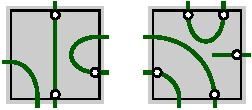
\includegraphics[]{pic-cells-2.pdf}
\end{center}

In joining tiles together to make a tiling we will
require adjacent tiles to agree on their shared boundary.
This will entail sequentially pairing symbols in the
words for adjacent tiles
and requiring that 
the {\tt in} and {\tt out} decorations are matched.
Because the word for a tile proceeds conter-clockwise
around the tile, this pairing will always reverse the
sequential order of the symbols of adjacent tiles.
For example, given the above two tiles we sequentially pair the 
$\bigl<_{\mbox{\tt out},2}\bigr>_{\mbox{\tt in},2}$ 
and $\bigr>_{\mbox{\tt out},4}\bigr>_{\mbox{\tt in},4}$
symbols with opposite order so that
$\bigl<_{\mbox{\tt out},2}\sim\bigr>_{\mbox{\tt in},4}$
and $\bigr>_{\mbox{\tt in},2} \sim \bigr>_{\mbox{\tt out},4}.$ 

Note that in general, this will allow us to store the multiple disjoint curve diagrams that cover the lattice.

For each piece-of-curve, apart from a head or tail, there is an associated 
number we call the \emph{turn number}. This counts the number
of ``right-hand turns'' the piece-of-curve makes as it
traverses the tile, with a ``left-hand turn'' counting as $-1.$
This number will take one of the values $-2, -1, 0, 1, 2:$
\begin{center}
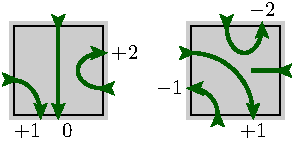
\includegraphics[]{pic-cells-3.pdf}
\end{center}


%
% ~~~~~~~~~~~~~~~~~~~~~~~~~~~~~~~~~~~~~~~~~~~~~~~~~~~~~~~~~~~~~~~~~~~~~~~~~~~~
%

\section{The paperclip algorithm}

In order to calculate the total charge of each tile, we must transport all anyons within the tile until they are neighbours along their curve. In doing so, it will be convenient to consider transporting these anyons by moving them along tile edges. This is equivalent to a ``refactoring'' of the fusion space, as described in Ref.~\cite{Burton2016}. We can further break down transport along the tile edge into a sequence of transports between neighbouring pieces of curve at that edge.
The origin and destination of such a path
now splits the curve diagram
into three disjoint pieces which we term
\emph{head}, \emph{body} and \emph{tail}, where
the head contains the endpoint of the curve, the tail
contains the beginning of the curve and the body is the remainder.
Here we consider transport forwards along the curve (from tail towards head), but the reverse case is analogous.
\begin{center}
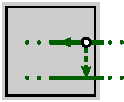
\includegraphics[]{pic-move-anyon.pdf}
\end{center}

This arrangement is equivalent (isotopic) to one of four 
``paperclips'', which we distinguish between by counting how
many \emph{right-hand turns} are made along the body of the curve diagram.
We also show an equivalent (isotopic) picture where the
curve diagram has been straightened, and the resulting distortion
in the anyon path:
\begin{center}
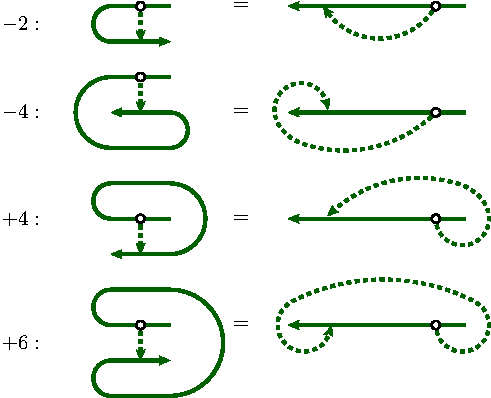
\includegraphics[]{pic-paperclip.pdf}
\end{center}
In order to perform the desired transport, we must braid the anyon under consideration around the other anyons along the curve diagram. Denoting the sequence of anyons along the head, body and tail, $H, B$ and $T,$
respectively, and using
$H^r, B^r$ and $T^r$ to denote the same anyons with the reversed order, the appropriate braiding transformation ($R$-move) can be read off for each
of the four paperclips:
\begin{align*}
-2:&\ R[B] \\
-4:&\ R[H^r]\ R[H]\ R[B] \\
+4:&\ R[B]\ R[T]\ R[T^r] \\
+6:&\ R[H^r]\ R[H]\ R[B]\ R[T]\ R[T^r] \\
\end{align*}
where notation such as $R[B]$ is understood as sequentially clockwise braiding around
each anyon in $B$. 

Once all the anyons within a tile have been brought into a sequential piece of the curve, their total charge can easily be read off by an appropriate $F$-move. This allows us to perform syndrome extraction, by repeating this procedure for each tile of the lattice.

%
% ~~~~~~~~~~~~~~~~~~~~~~~~~~~~~~~~~~~~~~~~~~~~~~~~~~~~~~~~~~~~~~~~~~~~~~~~~~~~
%

\section{Decoding and error-correction}

After the noise process is applied to the system,
the error correction routine attempts to annihilate all the anyons on the lattice in a way that does not affect the encoded information. It proceeds as a dialogue between the
decoder and the system. The syndrome extraction procedure provides information to the decoder, which suggests a recovery procedure, the results of which are found by a subsequent syndrome extraction step, and so on. This iterative procedure continues until the extracted syndrome is empty (i.e.~i.e. there are no remaining anyons on the lattice), or the decoder declares failure.
Here we show this in a process diagram, with time running up
the page:
\begin{center}
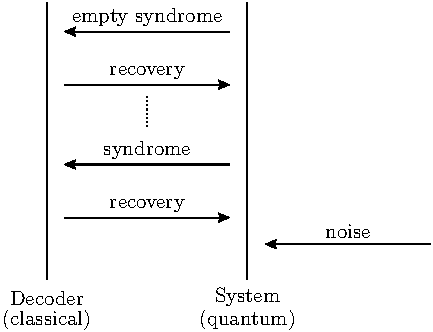
\includegraphics[]{pic-process.pdf}
\end{center}

So far we have discussed the simulation of the (quantum) system
and now we turn to the decoder algorithm. This is similar to other clustering-type decoders used in the literature~\cite{Bravyi2011}, in that it attempts to form and fuse together clusters of anyons on larger and larger length scales, declaring failure if anyons remain after fusion at the largest length scale. Our simulation also declares failure if at any point the curve diagrams describing the state of the system form a homologically non-trivial loop (span the lattice), this being a necessary condition for error-correction failure.

The structure of the error-correction routine is as follows, and will be illustrated by an example below.

\begin{verbatim}
 1:  def error_correct():
 2:      syndrome = get_syndrome()
 3:      
 4:      # build a cluster for each charge
 5:      clusters = [Cluster(charge) for charge in syndrome]
 6:  
 7:      # join any neighbouring clusters
 8:      join(clusters, 1)
 9:      
10:      while clusters:
11:      
12:          # find total charge on each cluster
13:          for cluster in clusters:
14:              fuse_cluster(cluster)
15:      
16:          # discard vacuum clusters
17:          clusters = [cluster for cluster in clusters if non_vacuum(cluster)]
18:      
19:          # grow each cluster by 1 unit
20:          for cluster in clusters:
21:              grow_cluster(cluster, 1)
22:      
23:          # join any intersecting clusters
24:          join(clusters, 0)
25:  
26:      # success !
27:      return True
\end{verbatim}

First, we show the result of the initial call to {\tt get\_syndrome()}, on line 2. This is computed using the syndrome extraction step as described above.
The locations of anyon charges are highlighted in red.
For each of these charges we build a {\tt Cluster}, on line 5.
Each cluster is shown as a gray shaded area.
\begin{center}
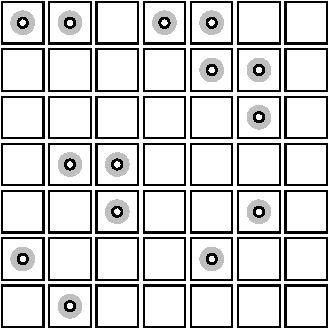
\includegraphics[]{pic-decode-0.pdf}
\end{center}
The next step is the call to {\tt join(clusters, 1)}, on line 8,
which joins clusters that are separated by at most one lattice
spacing. We now have seven clusters:
\begin{center}
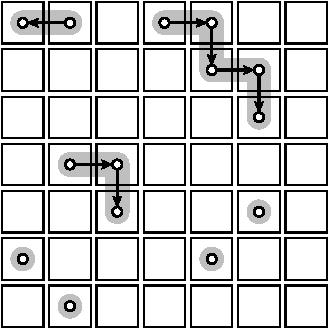
\includegraphics[]{pic-decode-1.pdf}
\end{center}
Each cluster is structured as a rooted tree, as indicated by
the arrows which point in the direction from the leaves to
the root of the tree. 
This tree structure is used in the call to {\tt fuse\_cluster()},
on line 14.
This moves anyons in the tree along the arrows to the root, 
fusing with the charge at the root. This movement of anyons is a physical recovery operation that is easily simulated by extending the curve diagram along the transport path, and moving the anyons along it.
\begin{center}
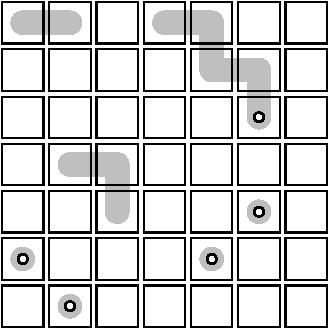
\includegraphics[]{pic-decode-2.pdf}
\end{center}
For each cluster, the charge is then measured using the syndrome extraction procedure, and the resulting charge at the root is taken as the charge of
that cluster. Any cluster with vacuum total charge is then discarded (line 17).
In our example, we find two clusters with vacuum charge and we discard these.
The next step is to grow the remaining clusters by one lattice spacing (line 20-21),
and join (merge) any overlapping clusters (line 24).
\begin{center}
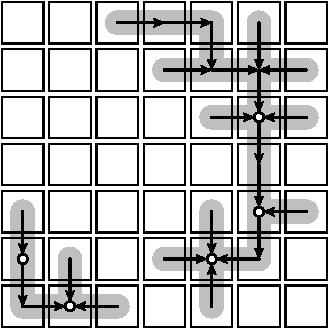
\includegraphics[]{pic-decode-3.pdf}
\end{center}
Note that we can choose the root of each cluster arbitrarily
since we are only interested in the total charge of each cluster, and also that for simplicity we have neglected the boundary of the lattice in
this example.

We repeat these steps of fusing, growing and then joining clusters (lines 10-24.)
If at any point this causes a topologically 
non-trivial operation, the simulation aborts and a failure
to decode is recorded.
Otherwise we eventually run out
of non-vacuum clusters, and the decoder succeeds (line 27).

By repeatedly performing this simulation of noise and error-correction on different sized lattices, and for different noise rates (or memory lifetimes), we are able to estimate the error-correction threshold for this type of system.

%------------------------------------------------------------------------------------------------------------%

%merlin.mbs apsrev4-1.bst 2010-07-25 4.21a (PWD, AO, DPC) hacked
%Control: key (0)
%Control: author (8) initials jnrlst
%Control: editor formatted (1) identically to author
%Control: production of article title (-1) disabled
%Control: page (0) single
%Control: year (1) truncated
%Control: production of eprint (0) enabled
\begin{thebibliography}{3}%
\makeatletter
\providecommand \@ifxundefined [1]{%
 \@ifx{#1\undefined}
}%
\providecommand \@ifnum [1]{%
 \ifnum #1\expandafter \@firstoftwo
 \else \expandafter \@secondoftwo
 \fi
}%
\providecommand \@ifx [1]{%
 \ifx #1\expandafter \@firstoftwo
 \else \expandafter \@secondoftwo
 \fi
}%
\providecommand \natexlab [1]{#1}%
\providecommand \enquote  [1]{``#1''}%
\providecommand \bibnamefont  [1]{#1}%
\providecommand \bibfnamefont [1]{#1}%
\providecommand \citenamefont [1]{#1}%
\providecommand \href@noop [0]{\@secondoftwo}%
\providecommand \href [0]{\begingroup \@sanitize@url \@href}%
\providecommand \@href[1]{\@@startlink{#1}\@@href}%
\providecommand \@@href[1]{\endgroup#1\@@endlink}%
\providecommand \@sanitize@url [0]{\catcode `\\12\catcode `\$12\catcode
  `\&12\catcode `\#12\catcode `\^12\catcode `\_12\catcode `\%12\relax}%
\providecommand \@@startlink[1]{}%
\providecommand \@@endlink[0]{}%
\providecommand \url  [0]{\begingroup\@sanitize@url \@url }%
\providecommand \@url [1]{\endgroup\@href {#1}{\urlprefix }}%
\providecommand \urlprefix  [0]{URL }%
\providecommand \Eprint [0]{\href }%
\providecommand \doibase [0]{http://dx.doi.org/}%
\providecommand \selectlanguage [0]{\@gobble}%
\providecommand \bibinfo  [0]{\@secondoftwo}%
\providecommand \bibfield  [0]{\@secondoftwo}%
\providecommand \translation [1]{[#1]}%
\providecommand \BibitemOpen [0]{}%
\providecommand \bibitemStop [0]{}%
\providecommand \bibitemNoStop [0]{.\EOS\space}%
\providecommand \EOS [0]{\spacefactor3000\relax}%
\providecommand \BibitemShut  [1]{\csname bibitem#1\endcsname}%
\let\auto@bib@innerbib\@empty
%</preamble>
\bibitem [{\citenamefont {Burton}(2016)}]{Burton2016}%
  \BibitemOpen
  \bibfield  {author} {\bibinfo {author} {\bibfnamefont {S.}~\bibnamefont
  {Burton}},\ }\href {http://arxiv.org/abs/1610.05384} {\  (\bibinfo {year}
  {2016})},\ \Eprint {http://arxiv.org/abs/arXiv:1610.05384} {arXiv:1610.05384}
  \BibitemShut {NoStop}%
\bibitem [{\citenamefont {Abramsky}(2007)}]{Abramsky2007}%
  \BibitemOpen
  \bibfield  {author} {\bibinfo {author} {\bibfnamefont {S.}~\bibnamefont
  {Abramsky}},\ }in\ \href@noop {} {\emph {\bibinfo {booktitle} {Mathematics of
  Quantum Computing and Technology}}},\ \bibinfo {editor} {edited by\ \bibinfo
  {editor} {\bibfnamefont {L.~K.}\ \bibnamefont {G.~Chen}}\ and\ \bibinfo
  {editor} {\bibfnamefont {S.}~\bibnamefont {Lomonaco}}}\ (\bibinfo
  {publisher} {Taylor \& Francis},\ \bibinfo {year} {2007})\ pp.\ \bibinfo
  {pages} {415--458}\BibitemShut {NoStop}%
\bibitem [{\citenamefont {Bravyi}\ and\ \citenamefont
  {Haah}(2013)}]{Bravyi2011}%
  \BibitemOpen
  \bibfield  {author} {\bibinfo {author} {\bibfnamefont {S.}~\bibnamefont
  {Bravyi}}\ and\ \bibinfo {author} {\bibfnamefont {J.}~\bibnamefont {Haah}},\
  }\href {\doibase 10.1103/PhysRevLett.111.200501} {\bibfield  {journal}
  {\bibinfo  {journal} {Phys. Rev. Lett.}\ }\textbf {\bibinfo {volume} {111}},\
  \bibinfo {pages} {200501} (\bibinfo {year} {2013})},\ \Eprint
  {http://arxiv.org/abs/1112.3252} {arXiv:1112.3252} \BibitemShut {NoStop}%
\end{thebibliography}%




\end{document}
